In questa sezione sono riportati i risultati ottenuti in termini di metriche fondamentali, la pipeline seguita per il training, evalutaion dei modelli e i grafici a confronto dell'andamento dell'accuracy su train e validation set durante l'addestramento. Il dettaglio verrà approfondito nella sezione apposita. 

\subsection{Configurazione Software/Hardware}
La configurazione con il quale sono stati effettuati i test è \textbf{Google Colab} utilizzando come tipo di runtime: Python3; Acceleratore hardware: GPU; Tipo di gpu: T4. Per l'implementazione, training dei modelli e valutazione dei modelli è stato utilizzato \textbf{Tensorflow} 2.12.0. La libreria utilizzata per i modelli preaddestrati di BERT è \textbf{Transformers} 4.29.2 di HuggingFace. Infine, \textbf{Sklearn} 1.2.2 per il preprocessing, train-test split e calcolo delle metriche.  

\subsection{Valutazione dei modelli}
\subsubsection{Metriche di valutazione}
Per la valutazioni dei modelli sono state utilizzate le metriche di Precision (Eq. \ref{eq:precisione}), Recall (Eq. \ref{eq:richiamo}), F1-Score (Eq. \ref{eq:f1_score}) e Accuracy (Eq. \ref{eq:accuracy}).
\begin{equation}
P = \frac{TP}{TP+FP} \label{eq:precisione}
\end{equation}

\begin{equation}
R = \frac{TP}{TP+FN} \label{eq:richiamo}
\end{equation}

\begin{equation}
\text{F1-Score} = 2 \times \frac{\text{Precision} \times \text{Recall}}{\text{Precision} + \text{Recall}} \label{eq:f1_score}
\end{equation}

\begin{equation}
\text{Accuracy} = \frac{TP + TN}{TP + TN + FP + FN} \label{eq:accuracy}
\end{equation}

\subsubsection{Comparazione e Training dei modelli}
Dopo aver effettuato il preprocessing dei dataset e la definizione dei modelli come da capitoli precenti la pipeline che si è andato a seguire 
(compresa anche di data preparation) è descritta in Figure \ref{fig:pipeline}.

\begin{figure}[!ht]
    \centering
    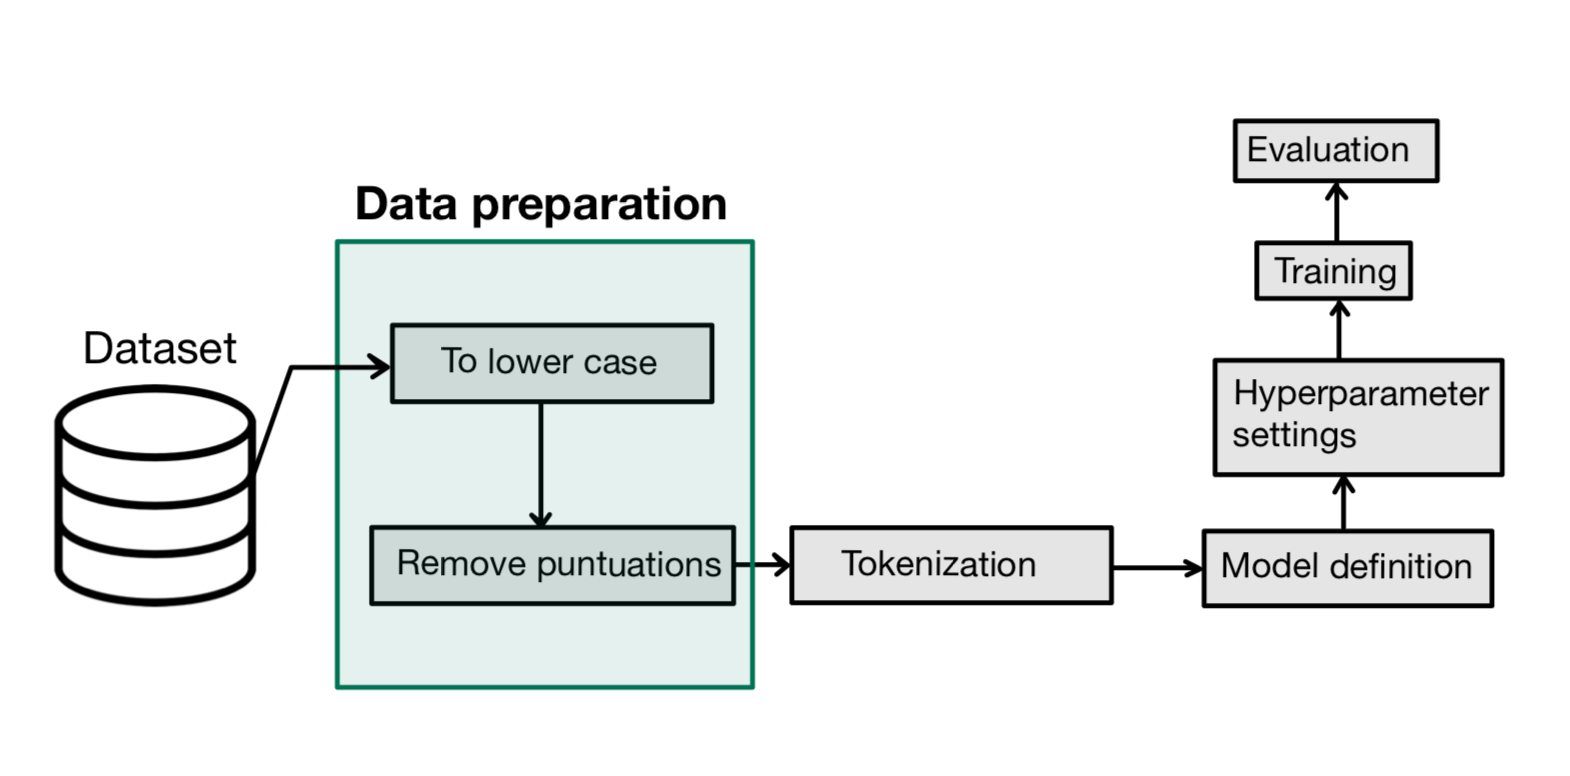
\includegraphics[width=12cm]{./images/pipeline.png}
    \caption{Implemented pipeline for Financial Sentiment Analysis}
    \label{fig:pipeline}
\end{figure}
\newpage
Inoltre la suddivisione in train-val-test set del dataset segue queste percentuali:
\begin{itemize}
    \item Train set: 70\%
    \item Validation set: 10\% del train set
    \item Test set: 30\%
\end{itemize}
Per il training di tutti e 4 i modelli impiegati nello studio del caso di studio sono state utilizzate due callbacks per cercare di evitare l'overfitting dei modelli durante il training, rispettivamente: early stopping e model checkpoint. Il model checkpoint  è stato impostato tale per cui andrà a salvare la versione del modello con la validation accuracy più alta durante il training. Mentre, l'early stopping terminerà il training se la validation accuracy non è migliorata per un numero di volte pari al parametro di patience.
L'optimizer utilizzato per tutti e 4 i modelli è Adam, dove per i modelli GloVe based sono stati utilizzati i parametri di default di Keras, mentre per le versioni di BERT il learning rate (lr) è pari a 5 $\times 10^{-5}$, $\epsilon = 1 \times 10^{-8}$ e clipnorm $= 1.0$.
Tutti gli altri iperparametri di training e le callbacks nello specifico sono indicate in Table \ref{tab:hyper-parameter}.
\newline
Infine, in Table \ref{tab:performance1}, \ref{tab:performance2} si possono vedere i valori, per entrambi i dataset considerati, di precision, recall e f1-score ottenuti in fase di validazione dei modelli. Tali valori sono stati presi tramite il metodo \codeinline{classificationReport()} di Sklearn, riportando come valori quelli con macroAVG, ovvero mediati sul numero delle classi. 

\begin{table}[!ht]
  \centering
  \begin{tabular}{c|c|c|c|c|c|c|c|c}
    Methods & Opimizer & Loss & Metric & Batch Size & Epochs & ES Patience\\
    \midrule
    GloVe+CNN & Adam & Sparse CCE & Accuracy & 32 & 100 & 5 \\
    GloVe+LSTM & Adam & Sparse CCE & Accuracy & 32 & 100 & 5\\
    FinBERT & Adam & CCE & Accuracy & 32 & 10 & 3\\
    DistilBERT & Adam & CCE & Accuracy & 32 & 10 & 3\\
    \bottomrule
  \end{tabular}
  \caption{Hyperparameters and compiling details of used methods}
  \label{tab:hyper-parameter}
\end{table}

\begin{table}[!ht]
  \centering
  \begin{tabular}{c|c|c|c|c}
    Methods & Precision (\%) & Recall (\%) & F1-Score (\%) & Accuracy (\%) \\
    \midrule
    GloVe+CNN & 77.38 & 73.47 & 75.14 & 79.27 \\
    GloVe+LSTM & 72.60 & 70.82 & 71.21 & 75.76 \\
    FinBERT & \textbf{84.52} & \textbf{83.22} & \textbf{83.82} & \textbf{85.54} \\
    DistilBERT & 84.49 & 81.14 & 82.66 & 84.44 \\
    \bottomrule
  \end{tabular}
  \caption{Performance comparization of implemented models on FinancialPhraseBank dataset}
  \label{tab:performance1}
\end{table}

\begin{table}[!ht]
  \centering
  \begin{tabular}{c|c|c|c|c}
    Methods & Precision (\%) & Recall (\%) & F1-Score (\%) & Accuracy (\%) \\
    \midrule
    GloVe+CNN & 63.76 & 60.84 & 61.28 & 73.22 \\
    GloVe+LSTM & 61.18 & 57.51 & 57.77 & 69.16 \\
    FinBERT & \textbf{72.11} & \textbf{74.45} & \textbf{73.07} & \textbf{78.18} \\
    DistilBERT & 69.60 & 68.58 & 68.97 & 76.47 \\
    \bottomrule
  \end{tabular}
  \caption{Performance comparization of implemented models on FinancialPhraseBank+FiQA dataset}
  \label{tab:performance2}
\end{table}

\newpage

\subsubsection{Grafici Training/Val Accuracy dei modelli su FinancialPhraseBank}
Come nella precedente sottosezione anche qui sono riportati i grafici della training/val accuracy dei vari modelli sul dataset FinancialPhraseBank.\newline
Rispettivamente del modello GloVe+CNN1d:
\begin{figure}[!ht]
    \centering
    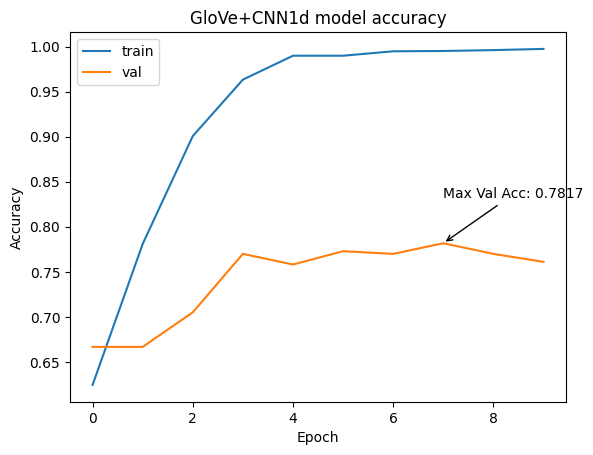
\includegraphics[width=12cm]{./images/plot_cnn.png}
    \caption{Plot of GloVe+CNN1d train/val accuracy}
\end{figure}
\newline
GloVe+LSTM:
\begin{figure}[!ht]
    \centering
    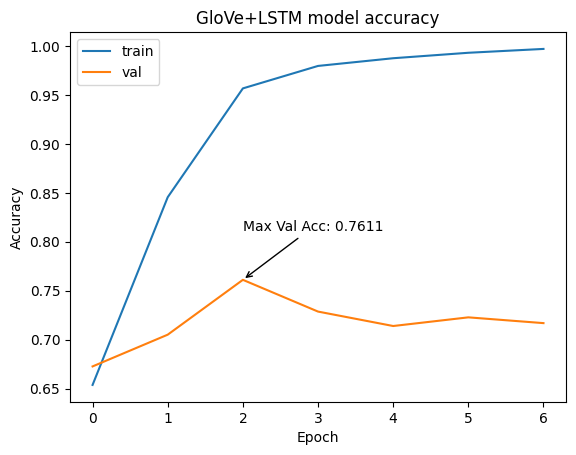
\includegraphics[width=11.5cm]{./images/plot_lstm.png}
    \caption{Plot of GloVe+LSTM train/val accuracy}
\end{figure}
\newline
\newpage
finBERT:
\begin{figure}[!ht]
    \centering
    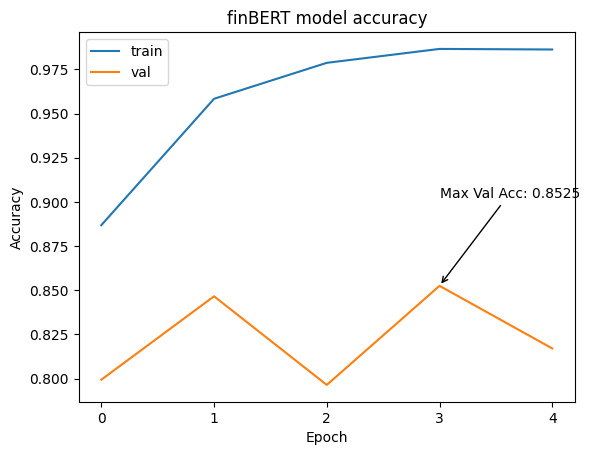
\includegraphics[width=12cm]{./images/plot_finBERT.png}
    \caption{Plot of FinBERT train/val accuracy}
\end{figure}
\newline
distilBERT:
\begin{figure}[!ht]
    \centering
    \includegraphics[width=12cm]{./images/plot_distilBERT.png}
    \caption{Plot of DistilBERT train/val accuracy}
\end{figure}

\newpage

\subsubsection{Grafici Training/Val Accuracy dei modelli su FinancialPhraseBank+FiQA}
Come nella precedente sottosezione anche qui sono riportati i grafici della training/val accuracy dei vari modelli sul dataset FinancialPhraseBank+FiQA.\newline
Rispettivamente del modello GloVe+CNN1d:
\begin{figure}[!ht]
    \centering
    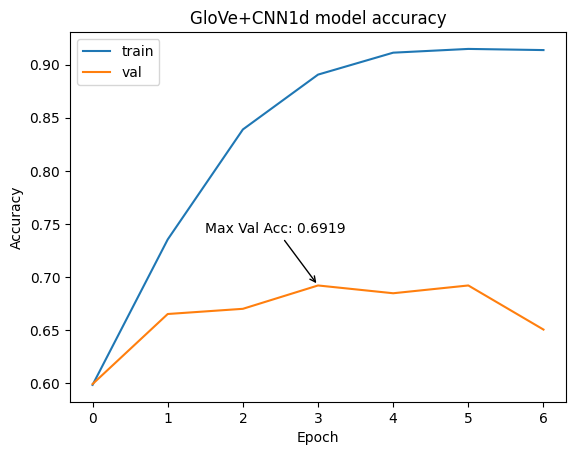
\includegraphics[width=12cm]{./images/acc_glove_cnn_2.png}
    \caption{Plot of GloVe+CNN1d train/val accuracy}
\end{figure}
\newline
GloVe+LSTM:
\begin{figure}[!ht]
    \centering
    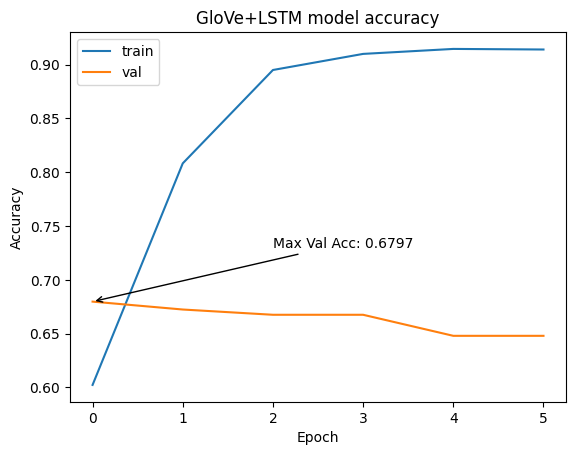
\includegraphics[width=11.5cm]{./images/acc_glove_lstm_2.png}
    \caption{Plot of GloVe+LSTM train/val accuracy}
\end{figure}
\newline
\newpage
finBERT:
\begin{figure}[!ht]
    \centering
    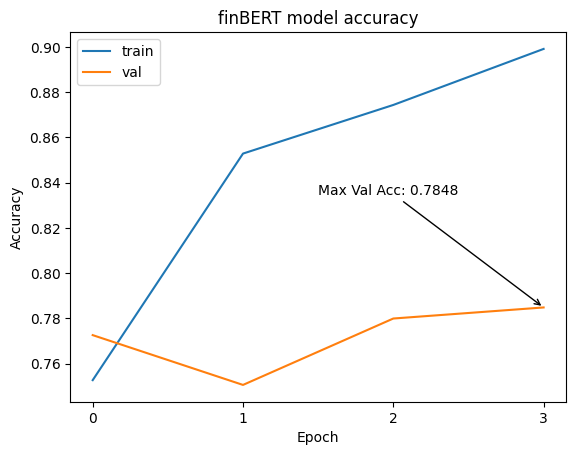
\includegraphics[width=12cm]{./images/acc_finBERT_2.png}
    \caption{Plot of FinBERT train/val accuracy}
\end{figure}
\newline
distilBERT:
\begin{figure}[!ht]
    \centering
    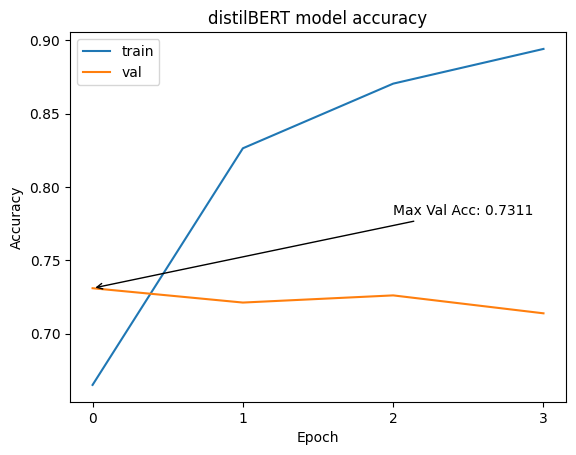
\includegraphics[width=12cm]{./images/acc_distilBERT_2.png}
    \caption{Plot of DistilBERT train/val accuracy}
\end{figure}

\newpage

\subsection{Output}
Di seguito sono riportate le previsioni ottenute in output dai relativi modelli sulle headline prese in esempio in \ref{section:1}:
    \begin{table}[!ht]
    \centering
    \caption{Example prediction of GloVe+CNN}
    \begin{tabular}{ccc}
      \toprule
          Headline &  Prediction & True label \\
          \midrule
          Positive news headline \ref{label:1} & neutral & positive \\
          Negative news headline & neutral & negative \\
          Neutral news headline & neutral & neutral \\
          \bottomrule
    \end{tabular}
  \end{table}

    \begin{table}[!ht]
    \centering
    \caption{Example prediction of GloVe+LSTM}
    \begin{tabular}{ccc}
      \toprule
          Headline &  Prediction & True label \\
          \midrule
          Positive news headline \ref{label:1} & positive & positive \\
          Negative news headline & negative & negative \\
          Neutral news headline & neutral & neutral \\
          \bottomrule
    \end{tabular}
  \end{table}

\begin{table}[!ht]
    \centering
    \caption{Example prediction of FinBERT}
    \begin{tabular}{ccc}
      \toprule
          Headline &  Prediction & True label \\
          \midrule
          Positive news headline \ref{label:1} & positive & positive \\
          Negative news headline & negative & negative \\
          Neutral news headline & neutral & neutral \\
          \bottomrule
    \end{tabular}
  \end{table}

  \begin{table}[!ht]
    \centering
    \caption{Example prediction of DistilBERT}
    \begin{tabular}{ccc}
      \toprule
          Headline &  Prediction & True label \\
          \midrule
          Positive news headline \ref{label:1} & positive & positive \\
          Negative news headline & negative & negative \\
          Neutral news headline & neutral & neutral \\
          \bottomrule
    \end{tabular}
  \end{table}
\newpage



